% ------------------------------------------------------------------------------
% TYPO3 CMS 7.5 - What's New - Chapter "Introduction" (Dutch Version)
%
% @author	Michael Schams <schams.net>
% @license	Creative Commons BY-NC-SA 3.0
% @link		http://typo3.org/download/release-notes/whats-new/
% @language	Dutch
% ------------------------------------------------------------------------------
% LTXE-CHAPTER-UID:		3a84d600-9fb67dda-31c4af65-dd7a4af5
% LTXE-CHAPTER-NAME:	Introduction
% ------------------------------------------------------------------------------

\section{Inleiding}
\begin{frame}[fragile]
	\frametitle{Inleiding}

	\begin{center}\huge{Inleiding}\end{center}
	\begin{center}\huge{\color{typo3darkgrey}\textbf{De feiten}}\end{center}

\end{frame}

% ------------------------------------------------------------------------------
% LTXE-SLIDE-START
% LTXE-SLIDE-UID:		6075d592-2ccf4301-19233322-9495ee57
% LTXE-SLIDE-ORIGIN:	81d53787-fb3806f0-841b4042-7033fad4 English
% LTXE-SLIDE-ORIGIN:	f1ea1041-2b6b2b81-f54b45c0-84265d6a German
% LTXE-SLIDE-TITLE:		TYPO3 CMS 7.5 - The Facts
% ------------------------------------------------------------------------------
\begin{frame}[fragile]
	\frametitle{Inleiding}
	\framesubtitle{TYPO3 CMS 7.5 - De feiten}

	\begin{itemize}
		\item Publicatiedatum: 29 september 2015
		\item Publicatietype: "Sprint Release"
		\item Visie: Omarm, Innoveer, Verspreid
		\item Primaire focus: Afronding
	\end{itemize}

	\begin{figure}
		
\includegraphics[width=0.95\linewidth]{Introduction/typo3cms75-banner.jpg}
	\end{figure}

\end{frame}

% ------------------------------------------------------------------------------
% LTXE-SLIDE-START
% LTXE-SLIDE-UID:		66f38f6e-3f0c844a-b0970f70-3ea51a74
% LTXE-SLIDE-ORIGIN:	a0327db8-b4a9bd42-f32515d0-87296684 English
% LTXE-SLIDE-ORIGIN:	5d8adc7d-af29cb46-4acd2255-27362935 German
% LTXE-SLIDE-TITLE:		System Requirements
% ------------------------------------------------------------------------------
\begin{frame}[fragile]
	\frametitle{Inleiding}
	\framesubtitle{Systeemeisen}

	\begin{itemize}
		\item PHP*:\tabto{2.2cm}v5.5.0 - v5.6.x
		\item MySQL:\tabto{2.2cm}v5.5.x - v5.6.x (geen strict mode)
		\item Schijfruimte:\tabto{2.2cm}min 200 MB
		\item PHP-instellingen:

			\begin{itemize}
				\item memory\_limit >= 128M
				\item max\_execution\_time >= 240s
				\item compilatieoptie \texttt{--disable-ipv6} \underline{niet} gebruiken
			\end{itemize}

		\item Backend vereist IE >= 9 of een andere moderne browser

	\end{itemize}

	\vspace{1cm}

	*) Meer details: \href{http://typo3.org/news/article/php-minimum-requirements-for-typo3-cms-7/}{PHP Minimum Requirements for TYPO3 CMS 7}

\end{frame}

% ------------------------------------------------------------------------------
% LTXE-SLIDE-START
% LTXE-SLIDE-UID:		75060275-f96b6318-3e76b8ed-7bbbc35a
% LTXE-SLIDE-ORIGIN:	c155d534-1a53682d-f56423dc-163111d3 English
% LTXE-SLIDE-ORIGIN:	6cad14bf-08874e74-1dd85333-e5c43a08 German
% LTXE-SLIDE-TITLE:		Development And Release Timeline
% ------------------------------------------------------------------------------
\begin{frame}[fragile]
	\frametitle{Inleiding}
	\framesubtitle{Ontwikkelings- en publicatietijdlijn}

	\begin{figure}
		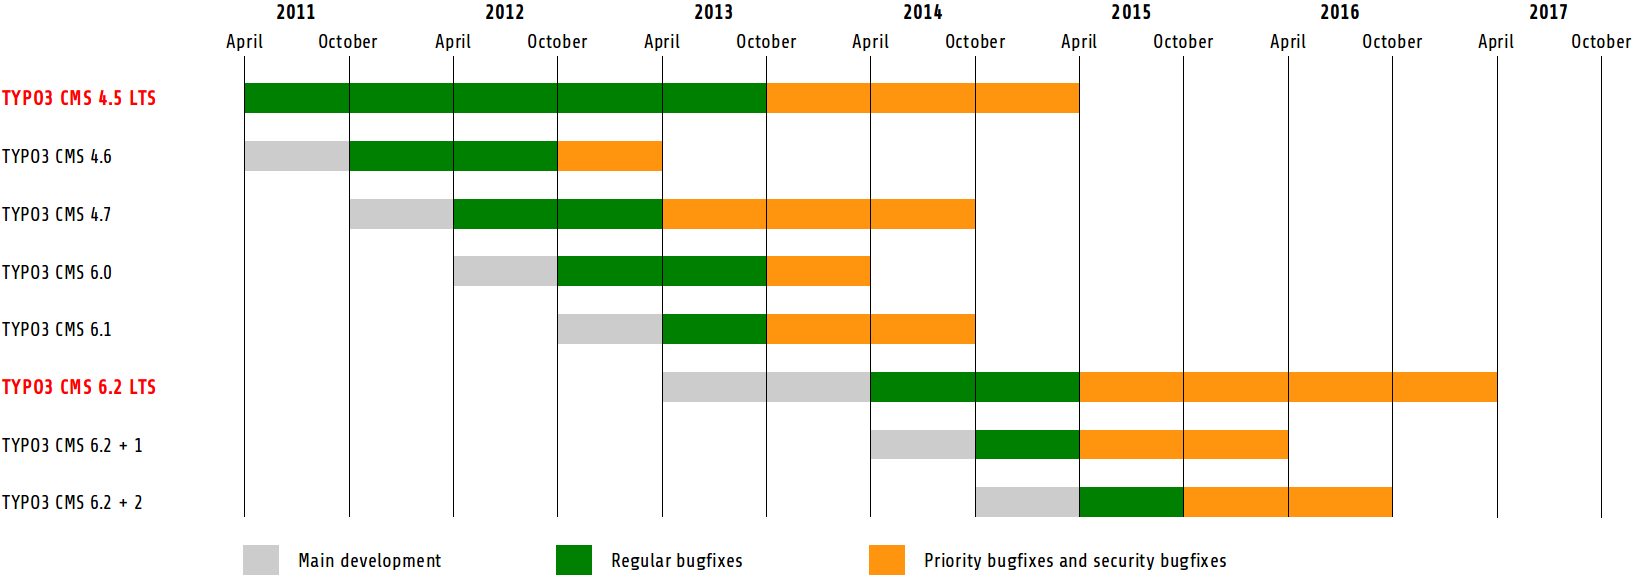
\includegraphics[width=0.90\linewidth]{Introduction/ReleaseAgenda.png}
	\end{figure}

\end{frame}

% ------------------------------------------------------------------------------
% LTXE-SLIDE-START
% LTXE-SLIDE-UID:		ce7ea23a-b1147d94-0971297a-8ac4fe18
% LTXE-SLIDE-ORIGIN:	83c1fb1c-ed592fa9-a2a279bd-be5cc800 English
% LTXE-SLIDE-ORIGIN:	387f7aeb-53ab533f-95427547-3aa76412 German
% LTXE-SLIDE-TITLE:		TYPO3 CMS Roadmap
% ------------------------------------------------------------------------------
\begin{frame}[fragile]
	\frametitle{Inleiding}
	\framesubtitle{TYPO3 CMS Roadmap}

	Geschatte publicatiedatum en primaire focus:

	\begin{itemize}
		\item v7.0 \tabto{1.1cm}02 dec 2014\tabto{3.4cm}Backend makeover deel 1
		\item v7.1 \tabto{1.1cm}24 feb 2015\tabto{3.4cm}Core opschonen en stroomlijnen
		\item v7.2 \tabto{1.1cm}28 apr 2015\tabto{3.4cm}Frontend
		\item v7.3 \tabto{1.1cm}16 jun 2015\tabto{3.4cm}Package Ecosysteem, Composer\newline
			\tabto{3.4cm}en Extensieafhandeling
		\item v7.4 \tabto{1.1cm}04 aug 2015\tabto{3.4cm}Backend Overhaul deel 2

		\item
			\begingroup
				\color{typo3orange}
					v7.5 \tabto{1.1cm}29 sep 2015\tabto{3.4cm}Afronding
			\endgroup

		\item v7 LTS \tabto{1.1cm}Okt/nov 2015\tabto{3.4cm}\textbf{TYPO3 CMS 7 LTS} (Long Term Release)
	\end{itemize}

	\smaller
		\url{https://typo3.org/typo3-cms/roadmap/}\newline
		\url{http://typo3.org/news/article/embrace-and-innovate-typo3-cms-7/}
	\normalsize

\end{frame}

% ------------------------------------------------------------------------------
% LTXE-SLIDE-START
% LTXE-SLIDE-UID:		2aafe392-8024d8b5-2742be9d-1d3b09cf
% LTXE-SLIDE-ORIGIN:	63decc15-57478e30-70c7ae99-27abd3c2 English
% LTXE-SLIDE-ORIGIN:	3b01edfd-6f06e241-2670b2ad-1b598b4e German
% LTXE-SLIDE-TITLE:		Installation
% ------------------------------------------------------------------------------
\begin{frame}[fragile]
	\frametitle{Inleiding}
	\framesubtitle{Installatie}

	\begin{itemize}
		\item Officiële installatieprocedure op Linux/Mac OS X\newline
			(DocumentRoot bijvoorbeeld \texttt{/var/www/site/htdocs}):
		\begin{lstlisting}
			$ cd /var/www/site
			$ wget --content-disposition get.typo3.org/7.5
			$ tar xzf typo3_src-7.5.0.tar.gz
			$ cd htdocs
			$ ln -s ../typo3_src-7.5.0 typo3_src
			$ ln -s typo3_src/index.php
			$ ln -s typo3_src/typo3
			$ touch FIRST_INSTALL
		\end{lstlisting}

		\item Symbolische koppelingen op Microsoft Windows:

			\begin{itemize}
				\item Gebruik \texttt{junction} met Windows XP/2000
				\item Gebruik \texttt{mklink} met Windows Vista en Windows 7
			\end{itemize}

	\end{itemize}
\end{frame}

% ------------------------------------------------------------------------------
% LTXE-SLIDE-START
% LTXE-SLIDE-UID:		374b6c9a-85778e17-0526cb70-765e0c60
% LTXE-SLIDE-ORIGIN:	12551741-9cb07199-fb3614d0-1a242a5f English
% LTXE-SLIDE-ORIGIN:	af099855-2b970b2b-89ed7d02-7219b2b9 German
% LTXE-SLIDE-TITLE:		Upgrade to TYPO3 CMS 7
% ------------------------------------------------------------------------------
\begin{frame}[fragile]
	\frametitle{Inleiding}
	\framesubtitle{Upgrade naar TYPO3 CMS 7.x}

	\begin{itemize}
		\item Upgrades alleen mogelijk van TYPO3 CMS 6.2 LTS
		\item TYPO3 CMS < 6.2 moet eerst worden geüpgrade naar TYPO3 CMS 6.2 LTS
	\end{itemize}

	\begin{itemize}

		\item Upgrade-instructies:\newline
			\smaller\url{http://wiki.typo3.org/Upgrade#Upgrading_to_7.5}\normalsize
		\item Officiële TYPO3-handleiding "TYPO3 Installation and Upgrading":
			\smaller\url{http://docs.typo3.org/typo3cms/InstallationGuide}\normalsize
		\item Algemene aanpak:
			\begin{itemize}
				\item Controleer minimale systeemeisen (PHP, MySQL, etc.)
				\item Inspecteer \textbf{deprecation\_*.log} in oude TYPO3-installatie
				\item Werk alle extensies bij naar de nieuwste versie
				\item Zet nieuwe bronbestanden neer en start\newline
					Installatie-module \textrightarrow Upgrade Wizard
				\item Check startmodule voor backend gebruikers (optioneel)
			\end{itemize}
	\end{itemize}

\end{frame}

% ------------------------------------------------------------------------------
